% !TEX root = ../main.tex

% 实验记录	
\begin{table}
	\renewcommand\arraystretch{1.7}
	\centering
	\begin{tabularx}{\textwidth}{|X|X|X|X|}
		\hline
		Major: & Physics & Grade: & 2022 \\
		\hline
		Name: & \textbf{杨舒云、戴鹏辉、朱政鑫、马万成} & Student number: & 22344020、22344016、22344019、22344018\\
		\hline
		Room temperature: & 26\degree C & Experimental location: & 四楼实验室 \\
		\hline
		Student Signature:& \textbf{In Attachment} & Score: &\\
		\hline
		Experiment time:& 2024/10/18 & Teacher's Signature:&\\
		\hline
	\end{tabularx}
\end{table}
\section{APL1-3 氦氖激光综合实验 \\ Experimental Record}


%---------------------------------------------------------------------
% 实验过程记录
\subsection{Content, Procedures \& Results}

% 操作步骤
\subsubsection{Operations}
实验具体操作由戴鹏辉22344016主导完成。
\begin{enumerate}
	\item 氦氖激光谐振腔调整与功率测量实验
	\begin{enumerate}
		\item 根据氦氖激光谐振腔调整与功率测量实验装配图(\cref{fig:apl18exp1})安装所有的器件。
		
		\begin{figure}[h!]
			\centering
			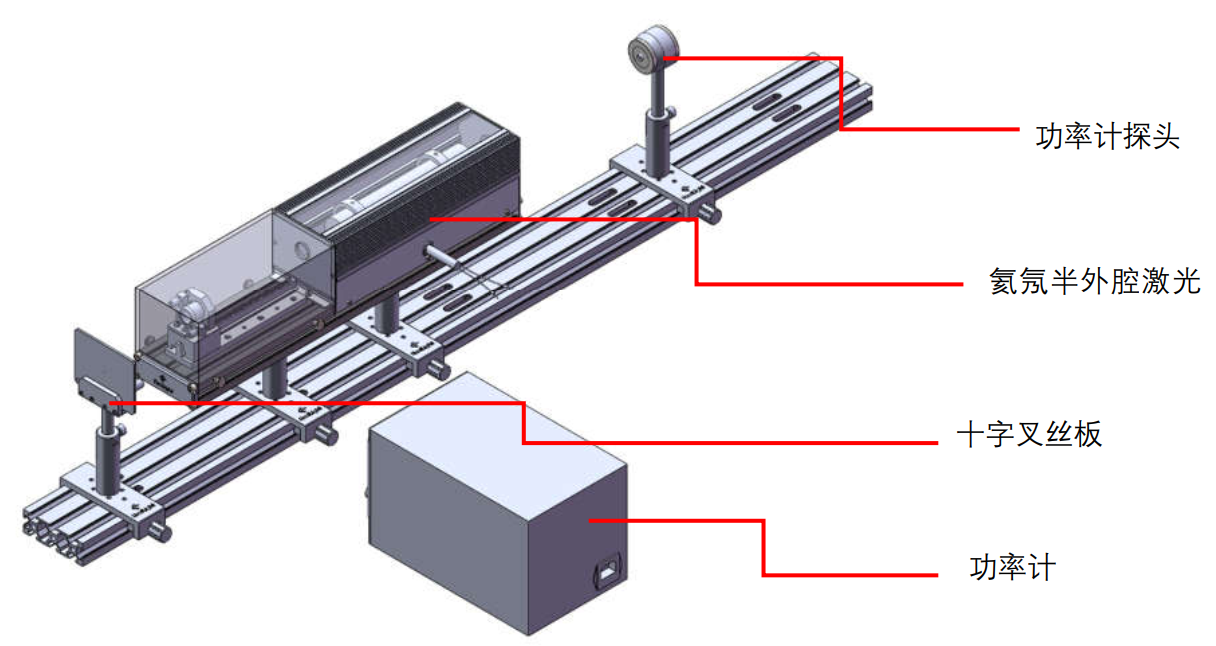
\includegraphics[width=0.5\linewidth]{images/APL1_8_Exp1}
			\caption{氦氖激光谐振腔调整与功率测量实验}
			\label{fig:apl18exp1}
		\end{figure}
		
		\item 使用台灯照亮十字叉丝板,叉丝线朝向半外腔激光器。
		
		\item 通过叉丝板中心小孔,目视氦氖激光器毛细腔。调整叉丝板小孔的位置,使得操作人可以目视到毛细管另一端腔片上的极亮斑,并将亮斑调整到毛细管中心。
		
		\item 调整半外腔激光器后腔镜旋钮,此时操作人通过叉丝板小孔可以看见经照亮的十字叉丝板图案反射到半外腔激光器后腔镜表面上的像,调整后腔镜镜架旋钮,将叉丝像交点与毛细管内亮斑重合。
		
		\item 反复调节,直至激光器发光。
		
		\item 使用功率计测量激光的功率。微调后腔镜镜架旋钮,直至激光器功率达到最大值。
		
		\item 改变后腔镜位置后,重复 2-6 步操作。
		
		\item 更换其他曲率的后腔镜后重复 2-7 步操作。
		
		\item 分别使用三种曲率的后腔镜,每种后腔镜更换三个位置,记录每处功率最大值。测量得到的数据如\cref{tab:exp1}所示。
	\end{enumerate}
	
	\item 激光横模变换与参数测量实验
	\begin{enumerate}
		\item 根据实验 1 的方法调出光。
		
		\begin{figure}[h!]
			\centering
			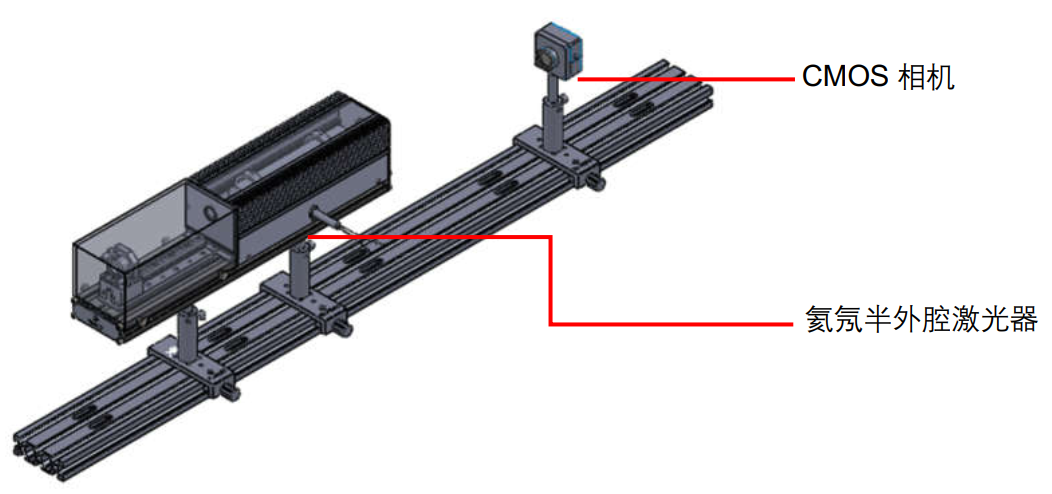
\includegraphics[width=0.5\linewidth]{images/APL1_8_Exp2}
			\caption{不同模式分析实验}
			\label{fig:apl18exp2}
		\end{figure}
		
		\item 连接相机,打开光斑分析软件观察光斑形态,确定激光模式。
		
		\item 通过调节安装后腔镜的齿轮齿条平移台以及后腔镜上的俯仰偏摆旋钮来改变激光器腔长,从而改变激光器的模式。
		
		\item 用光斑分析软件测量不同模式下光斑的宽度,用这些数据计算不同模式下的激光高斯光束参数。
		
		\item 把氦氖激光器更换成半导体激光器,再次对光斑进行测量,并分析半导体激光器的特性。
		
		\item 实验测量得到的数据如\cref{tab:exp2-1}、\cref{tab:exp2-2}和\cref{tab:exp2-3}所示。
	\end{enumerate}
	
	\item 高斯光束基本参数测量实验
	
	通过软件分析 CCD 上的光斑的光束半径,手动移动 CCD 的位置,可以测量得到高斯光束的光斑直径变化曲线。通过分析该曲线,可以计算出高斯光束的光腰半径、发散角、瑞利长度等参数,并分析出光束质量因子。
	
	\begin{figure}[h!]
		\centering
		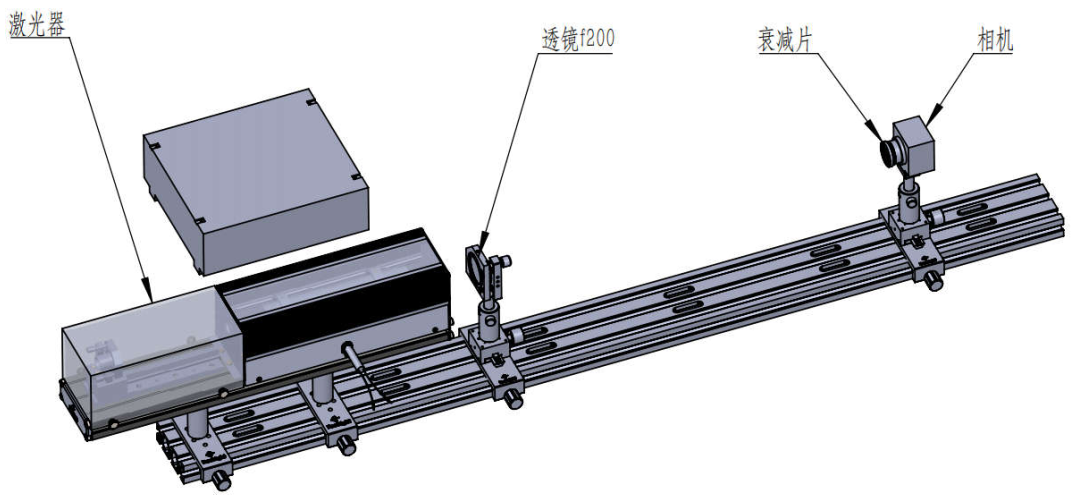
\includegraphics[width=0.5\linewidth]{images/APL1_8_Exp34}
		\caption{高斯光束基本参数的测量实验和高斯光束的传播特性实验}
		\label{fig:apl18exp34}
	\end{figure}
	
	\begin{enumerate}
		\item 搭建光路,先不放透镜。
		
		\item 打开相关软件并检查CCD拍摄。
		
		\item 调节光束光轴与 CCD 同轴。
		
		\item 透镜(f200mm)的放置,并调整光束的光轴与原光轴重合。
		
		\item 观察高斯光束的光束半径随距离的变化,并绘制距离-光束半径曲线。
		
		\item 实验软件截图如\cref{fig:apl18exp3printscreen}所示。
	\end{enumerate}
	
	\item 高斯光束的传播特性实验
	
	通过测量高斯光束的光束直径随相机位置变化曲线的方法,根据实验数据能够计算出氦氖激光器输出激光在各个位置处的 q 参数。我们首先测量激光器直接输出的高斯光束的光斑直径变化曲线,并计算出不同位置(测量范围内与外推到测量范围以外)的 q 参数,从而了解高斯光束的传播规律。接着在光路中放置透镜,测量加入透镜后光束的光斑直径变化曲线的变化,并用 q 参数方法分析透镜对光束的变换作用。
	\begin{enumerate}
		\item 搭建光路,先不放透镜。
		
		\item 打开氦氖激光器,在软件界面中可以浏览 CCD 拍摄的图像。
		
		\item 调节光束光轴与 CCD 同轴。
		
		\item 测量不加透镜激光自由传输时,激光器输出的高斯光束的光束半径随距离的变化曲线。
		
		\item 透镜(f200mm)的放置,并调整光束的光轴与原光轴重合。
		
		\item 测量加入透镜(f200mm)后高斯光束的光束半径随距离的变化曲线。
		
		\item 对比添加透镜前后的 q 参数的变化($q_in$ 和 $q_out$),分析透镜对于光束的变换,研究薄透镜对高斯光束的聚焦作用。
		
		\item 实验软件截图如\cref{fig:apl18exp4printscreen}和\cref{fig:apl18exp4printscreent}所示。
	\end{enumerate}
\end{enumerate}	

% 实验结果
\subsubsection{Display}
由马万成22344018主导,我们实验测量得到的数据如下。
\begin{enumerate}
	\item 氦氖激光谐振腔调整与功率测量实验
	
	\begin{table}[h!]
		\centering
		\renewcommand{\arraystretch}{1.5} % 调整行高
		\caption{不同曲率后腔镜在不同位置的功率最大值记录表}
		\label{tab:exp1}
		\begin{tabular}{|c|c|c|c|}
			\hline
			\textbf{后腔镜曲率/功率/位置} & \textbf{位置1(0cm)} & \textbf{位置2(-20cm)} & \textbf{位置3(-40cm)} \\ \hline
			R500 & 2.000 & 2.100 & 2.300 \\ \hline
			R1000 & 2.153 & 2.200 & 2.280 \\ \hline
			R2000 & 1.300 & 1.200 & 1.100 \\ \hline
		\end{tabular}
	\end{table}
	
	\item 激光横模变换与参数测量实验
	
	\begin{table}[htbp]
		\centering
		\renewcommand{\arraystretch}{1.5} % 调整行高
		\caption{单模He-Ne激光光斑宽度的测量\quad 单位:(mm)}
		\label{tab:exp2-1}
		\begin{tabular}{|c|c|c|c|c|c|c|c|}
			\hline
			\textbf{测量位置(按光具座刻度/cm)} & \textbf{60} & \textbf{65} & \textbf{70} & \textbf{75} & \textbf{80} & \textbf{85} & \textbf{90} \\ \hline
			\textbf{水平宽度(软件上标记为a/mm)} & 0.5505 & 0.6038 & 0.8814 & 0.7040 & 0.7866 & 0.8561 & 0.9410 \\ \hline
			\textbf{垂直宽度(软件上标记为b/mm)} & 0.6517 & 0.7545 & 0.6809 & 0.9414 & 1.0507 & 1.1748 & 1.2908 \\ \hline
		\end{tabular}
	\end{table}
	
	\begin{table}[htbp]
		\centering
		\renewcommand{\arraystretch}{1.5} % 调整行高
		\caption{多模He-Ne激光光斑宽度的测量\quad 单位:(mm)}
		\label{tab:exp2-2}
		\begin{tabular}{|c|c|c|c|c|c|c|c|}
			\hline
			\textbf{测量位置(光具座/cm)} & \textbf{60} & \textbf{65} & \textbf{70} & \textbf{75} & \textbf{80} & \textbf{85} & \textbf{90} \\ \hline
			\textbf{水平宽度(a/mm)} & 1.0166 & 1.1136 & 1.2791 & 1.3891 & 1.6424 & 1.7512 & 2.0274 \\ \hline
			\textbf{垂直宽度(b/mm)} & 0.7482 & 0.8052 & 0.9341 & 1.0101 & 1.1846 & 1.2462 & 1.4523 \\ \hline
		\end{tabular}
	\end{table}
	
	\begin{table}[htbp]
		\centering
		\renewcommand{\arraystretch}{1.5} % 调整行高
		\caption{半导体激光光斑宽度的测量\quad 单位:(mm)}
		\label{tab:exp2-3}
		\begin{tabular}{|c|c|c|c|c|c|c|c|}
			\hline
			\textbf{测量位置(光具座/cm)} & \textbf{60} & \textbf{65} & \textbf{70} & \textbf{75} & \textbf{80} & \textbf{85} & \textbf{90} \\ \hline
			\textbf{水平宽度(a/mm)} & 1.6458 & 1.6965 & 1.6894 & 1.7284 & 1.6936 & 1.5853 & 1.7277 \\ \hline
			\textbf{垂直宽度(b/mm)} & 0.9598 & 1.1150 & 1.1325 & 1.1620 & 1.1410 & 1.0788 & 1.1387 \\ \hline
		\end{tabular}
	\end{table}
	
	\item 高斯光束基本参数测量实验
	
	\begin{figure}[h!]
		\centering
		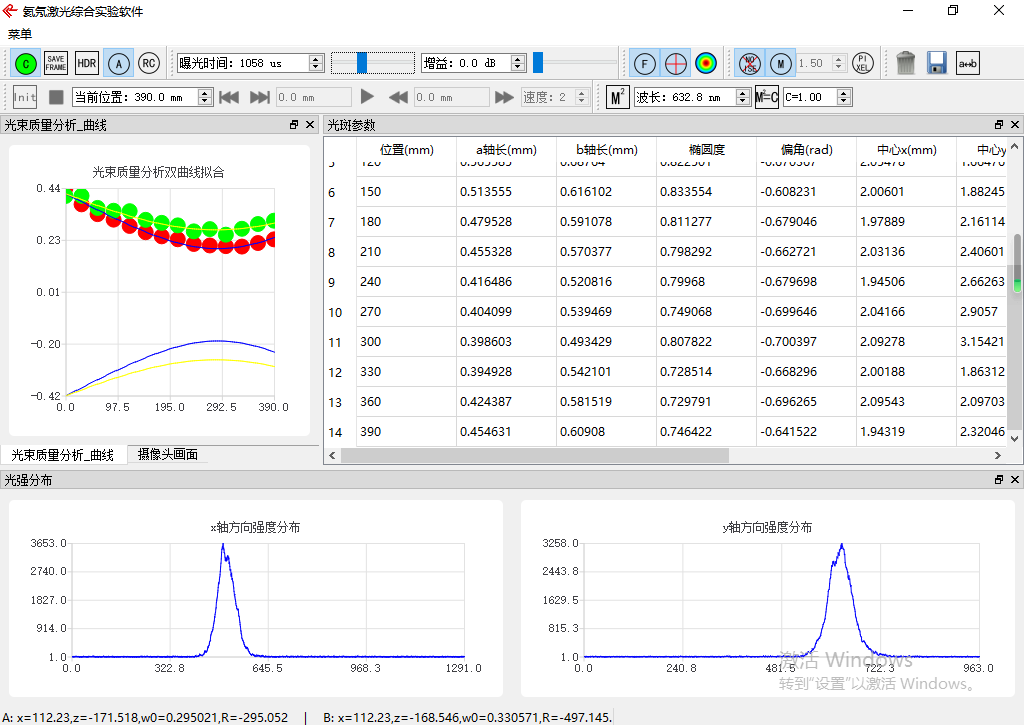
\includegraphics[width=0.7\linewidth]{images/APL1_8_exp3_printscreen}
		\caption{高斯光束基本参数测量实验:实验软件截图}
		\label{fig:apl18exp3printscreen}
	\end{figure}
	
	\item 高斯光束的传播特性实验
	
	\begin{figure}[h!]
		\centering
		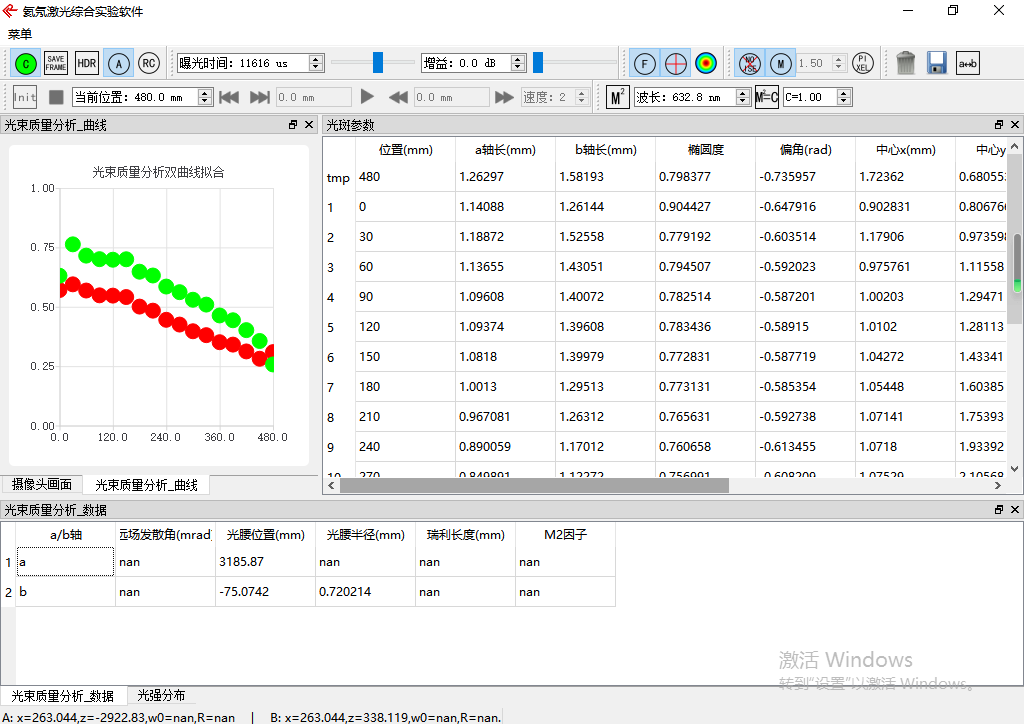
\includegraphics[width=0.7\linewidth]{images/APL1_8_exp4_printscreen}
		\caption{高斯光束的传播特性实验:实验软件截图(无透镜)}
		\label{fig:apl18exp4printscreen}
	\end{figure}
	
	\begin{figure}[h!]
		\centering
		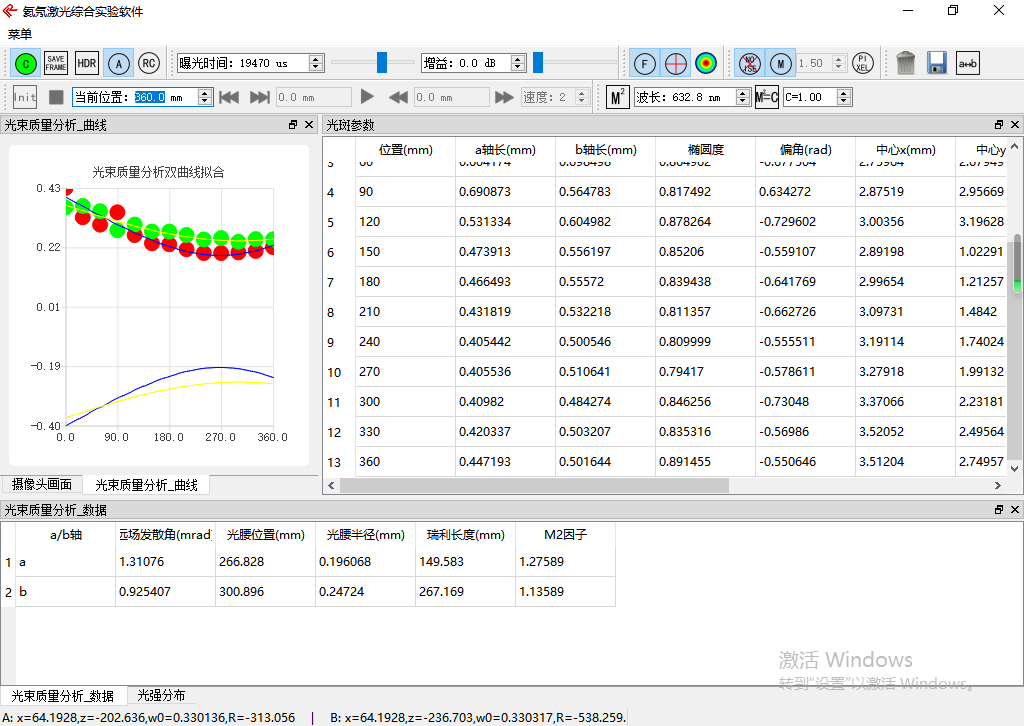
\includegraphics[width=0.7\linewidth]{images/APL1_8_exp4_printscreenT}
		\caption{高斯光束的传播特性实验:实验软件截图(加透镜)}
		\label{fig:apl18exp4printscreent}
	\end{figure}
	
\end{enumerate}

%---------------------------------------------------------------------
% 原始数据
\subsection{Original Data}
The original data in the experimental notebook is shown in \cref{fig:d8-originaldata-1} (signed).

\begin{figure}[htbp]
	\centering
	\includegraphics[width=0.7\linewidth]{APL1_8_original_data.jpg}
	\caption{原始数据记录}
	\label{fig:d8-originaldata-1}
\end{figure}

%See the \textbf{Attachment} section for the clean of the experimental bench desktop (%\cref{}).

Other raw data are shown in \cref{fig:apl18exp3printscreen}, \cref{fig:apl18exp4printscreen}, \cref{fig:apl18exp4printscreent} and \textbf{Attachment}.


%---------------------------------------------------------------------
% 问题记录
\subsection{Difficulties}
实验中遇到的困难和问题以及做实验的经验教训总结如下(由马万成22344018总结):
\begin{enumerate}
	\item 在调制激光器后腔镜使激光器发光中,激光器本身不水平,或者光学轨道不水平,使得原本应该十字叉丝与亮斑重合处严重下偏,在调光中耗费很多时间;
	\item 改变后腔镜曲率进行实验,越大的越难以调制出激光,这对实验仪器规整度要求太高;
	\item 调节激光模式中,高斯基模难以调出符合预期的模式,多是各种模式的叠加态;
	\item 光学轨道不水平,以及相机镜头的俯仰偏离,在改变镜头位置下,难以确保光斑始终在镜头中心;
	\item 由于基模调制质量的不同,数据拟合的质量也会有所不同,所得曲线不一定符合理论预期。
\end{enumerate}
% ---